\documentclass[11pt]{article}
\usepackage[textwidth=18.0cm, textheight=23.0cm, top=2.0cm]{geometry}
\usepackage{pst-all}
\usepackage{amssymb}
\usepackage{tikz}
\usepackage{underscore}\begin{document}
\pagestyle{empty}


ClassName: \underline{\textbf{Class_05.2bp-9}}
\par
BinSize: \underline{\textbf{100 × 100}}
\par
ReduceSize: \underline{\textbf{100 × 100}}
\par
TypeNum: \underline{\textbf{20}}
\par
Num: \underline{\textbf{20}}
\par
OutS: \underline{\textbf{80000}}
\par
InS: \underline{\textbf{58413}}
\par
Rate: \underline{\textbf{0.730}}
\par
UB: \underline{\textbf{8}}
\par
LB0: \underline{\textbf{8}}
\par
LB: \underline{\textbf{8}}
\par
LBWithCut: \underline{\textbf{8}}
\par
NodeCut: \underline{\textbf{0}}
\par
ExtendedNodeCnt: \underline{\textbf{1}}
\par
GenNodeCnt: \underline{\textbf{1}}
\par
PrimalNode: \underline{\textbf{0}}
\par
ColumnCount: \underline{\textbf{8}}
\par
TotalCutCount: \underline{\textbf{0}}
\par
RootCutCount: \underline{\textbf{0}}
\par
LPSolverCnt: \underline{\textbf{1}}
\par
PricingSolverCnt: \underline{\textbf{0}}
\par
BranchAndBoundNum: \underline{\textbf{1}}
\par
isOpt: \underline{\textbf{true}}
\par
TimeOnPrimal: \underline{\textbf{0.000 s}}
\par
TimeOnPricing: \underline{\textbf{0.000 s}}
\par
TimeOnRmp: \underline{\textbf{0.078 s}}
\par
TotalTime: \underline{\textbf{0.156 s}}
\par
\newpage



\begin{tikzpicture}[shorten >=1pt,scale=1.0,every node/.style={scale=1.0},->]
\tikzstyle{vertex}=[circle,fill=black!25,minimum size=14pt,inner sep=0pt]
\filldraw[fill=gray!40!white, draw=black] (0,0) rectangle (15.0,15.0);
\foreach \name/\x/\y/\w/\h in {100x95/0.0/0.0/15.0/14.25}
\filldraw[fill=white!40!white, draw=black] (\x,\y) rectangle node[draw] (\name) {\name} ++(\w,\h);
\end{tikzpicture}


w =100 , h =95 , x =0 , y =0 , v =9500
\par
\newpage


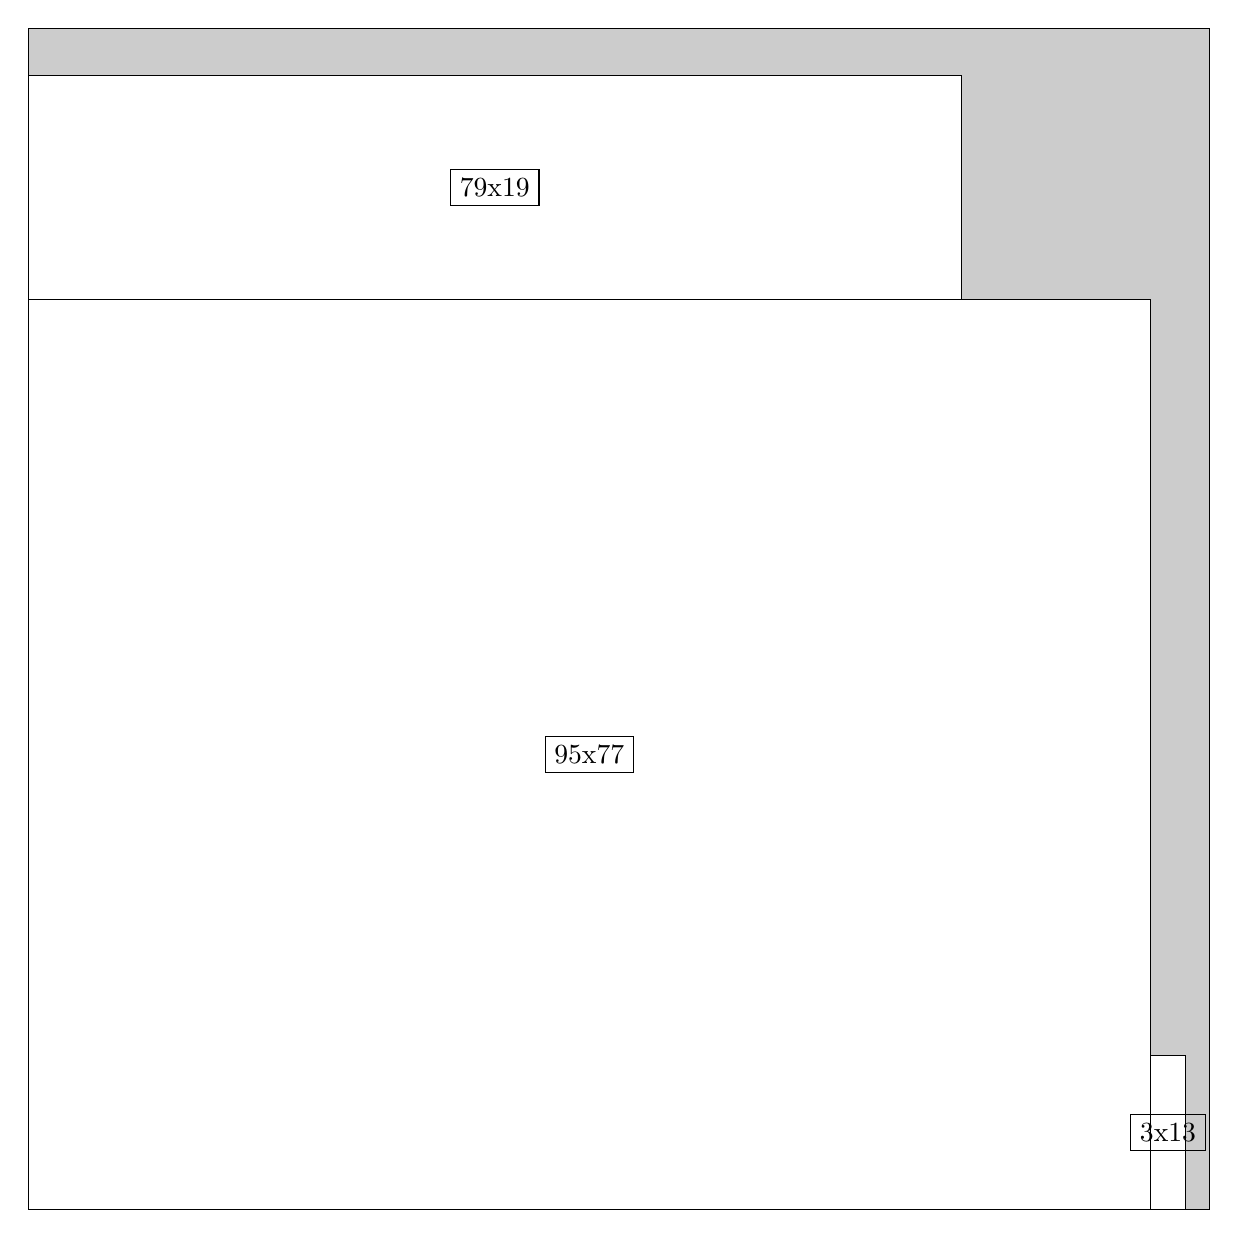
\begin{tikzpicture}[shorten >=1pt,scale=1.0,every node/.style={scale=1.0},->]
\tikzstyle{vertex}=[circle,fill=black!25,minimum size=14pt,inner sep=0pt]
\filldraw[fill=gray!40!white, draw=black] (0,0) rectangle (15.0,15.0);
\foreach \name/\x/\y/\w/\h in {95x77/0.0/0.0/14.25/11.549999999999999,79x19/0.0/11.549999999999999/11.85/2.85,3x13/14.25/0.0/0.44999999999999996/1.95}
\filldraw[fill=white!40!white, draw=black] (\x,\y) rectangle node[draw] (\name) {\name} ++(\w,\h);
\end{tikzpicture}


w =95 , h =77 , x =0 , y =0 , v =7315
\par
w =79 , h =19 , x =0 , y =77 , v =1501
\par
w =3 , h =13 , x =95 , y =0 , v =39
\par
\newpage


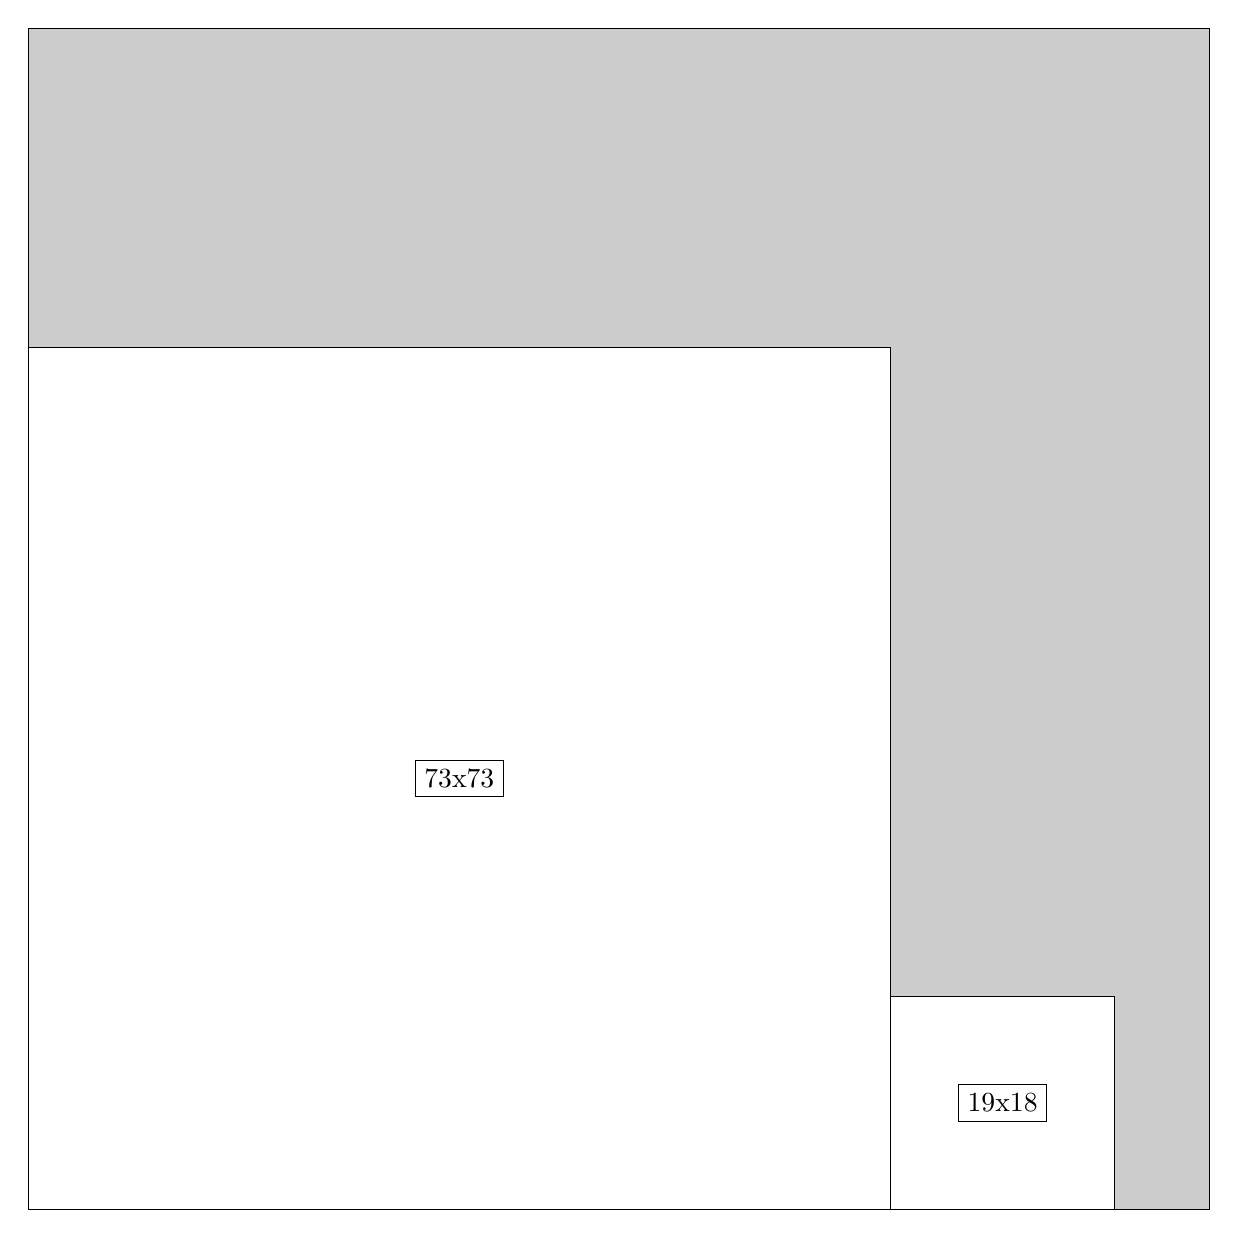
\begin{tikzpicture}[shorten >=1pt,scale=1.0,every node/.style={scale=1.0},->]
\tikzstyle{vertex}=[circle,fill=black!25,minimum size=14pt,inner sep=0pt]
\filldraw[fill=gray!40!white, draw=black] (0,0) rectangle (15.0,15.0);
\foreach \name/\x/\y/\w/\h in {73x73/0.0/0.0/10.95/10.95,19x18/10.95/0.0/2.85/2.6999999999999997}
\filldraw[fill=white!40!white, draw=black] (\x,\y) rectangle node[draw] (\name) {\name} ++(\w,\h);
\end{tikzpicture}


w =73 , h =73 , x =0 , y =0 , v =5329
\par
w =19 , h =18 , x =73 , y =0 , v =342
\par
\newpage


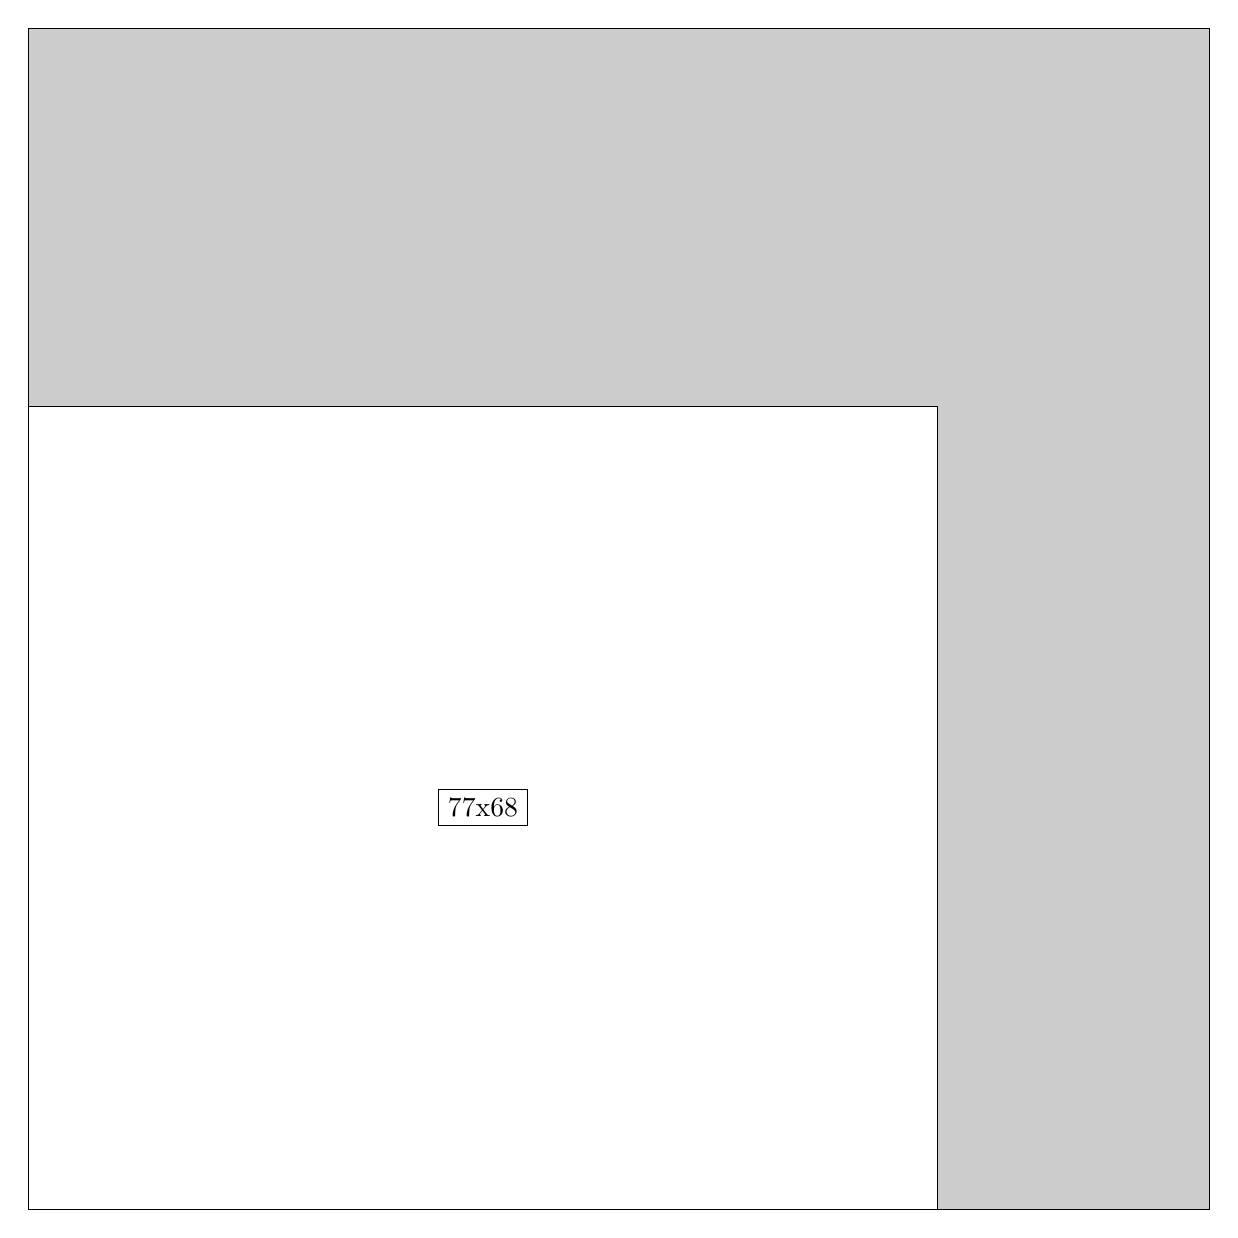
\begin{tikzpicture}[shorten >=1pt,scale=1.0,every node/.style={scale=1.0},->]
\tikzstyle{vertex}=[circle,fill=black!25,minimum size=14pt,inner sep=0pt]
\filldraw[fill=gray!40!white, draw=black] (0,0) rectangle (15.0,15.0);
\foreach \name/\x/\y/\w/\h in {77x68/0.0/0.0/11.549999999999999/10.2}
\filldraw[fill=white!40!white, draw=black] (\x,\y) rectangle node[draw] (\name) {\name} ++(\w,\h);
\end{tikzpicture}


w =77 , h =68 , x =0 , y =0 , v =5236
\par
\newpage


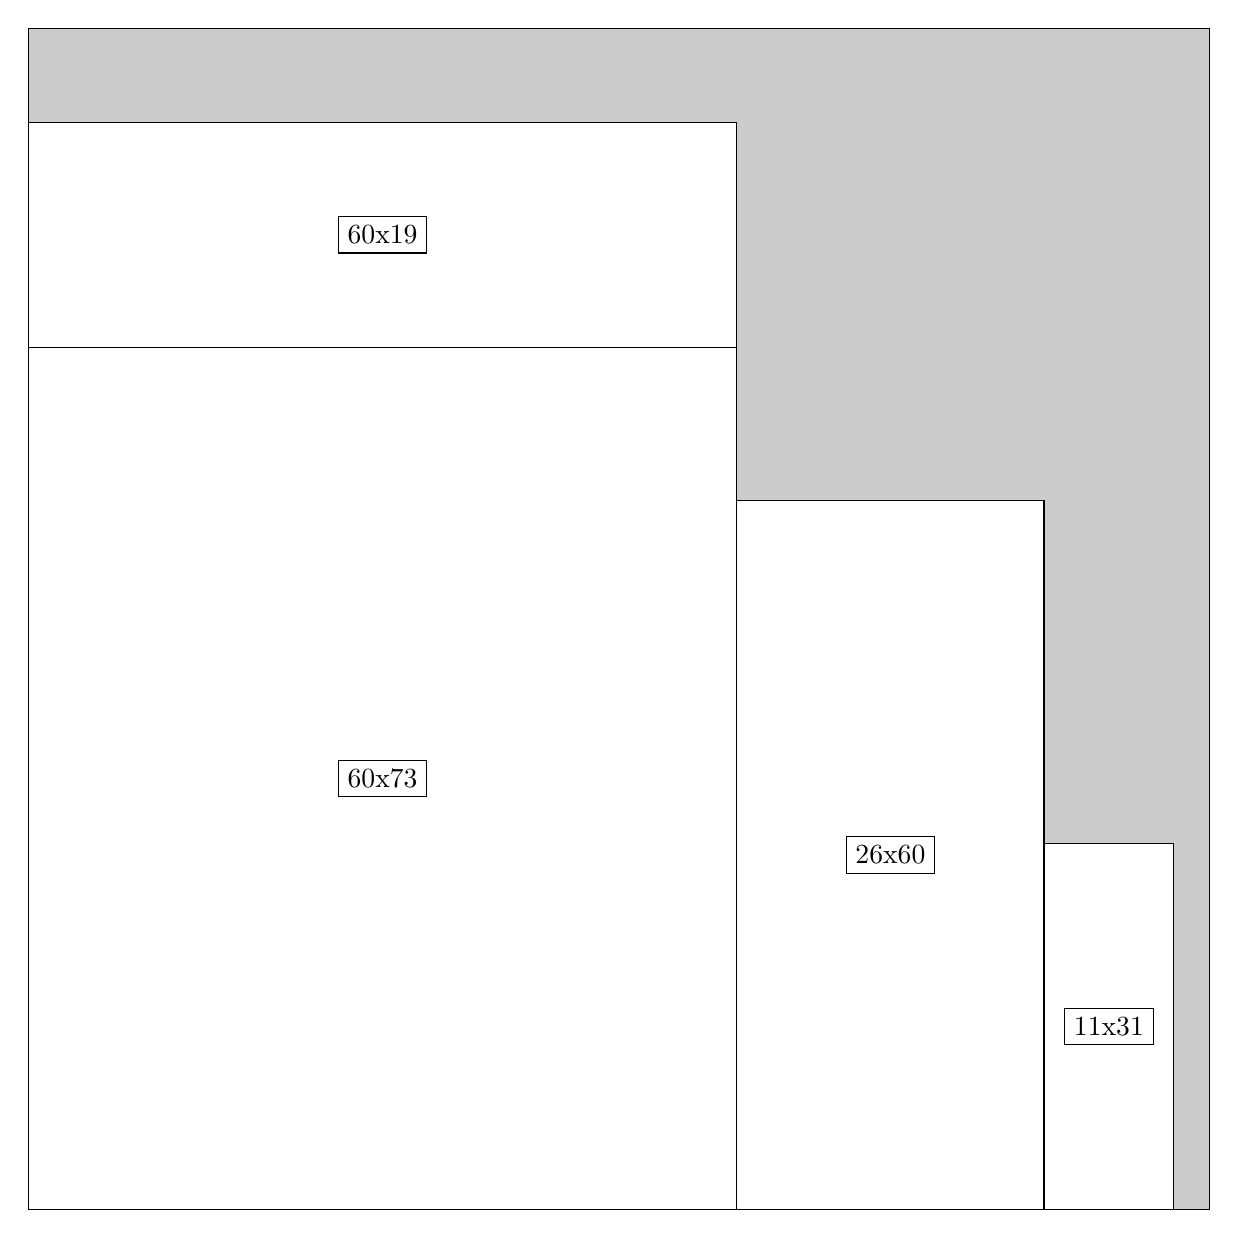
\begin{tikzpicture}[shorten >=1pt,scale=1.0,every node/.style={scale=1.0},->]
\tikzstyle{vertex}=[circle,fill=black!25,minimum size=14pt,inner sep=0pt]
\filldraw[fill=gray!40!white, draw=black] (0,0) rectangle (15.0,15.0);
\foreach \name/\x/\y/\w/\h in {60x73/0.0/0.0/9.0/10.95,26x60/9.0/0.0/3.9/9.0,60x19/0.0/10.95/9.0/2.85,11x31/12.9/0.0/1.65/4.6499999999999995}
\filldraw[fill=white!40!white, draw=black] (\x,\y) rectangle node[draw] (\name) {\name} ++(\w,\h);
\end{tikzpicture}


w =60 , h =73 , x =0 , y =0 , v =4380
\par
w =26 , h =60 , x =60 , y =0 , v =1560
\par
w =60 , h =19 , x =0 , y =73 , v =1140
\par
w =11 , h =31 , x =86 , y =0 , v =341
\par
\newpage


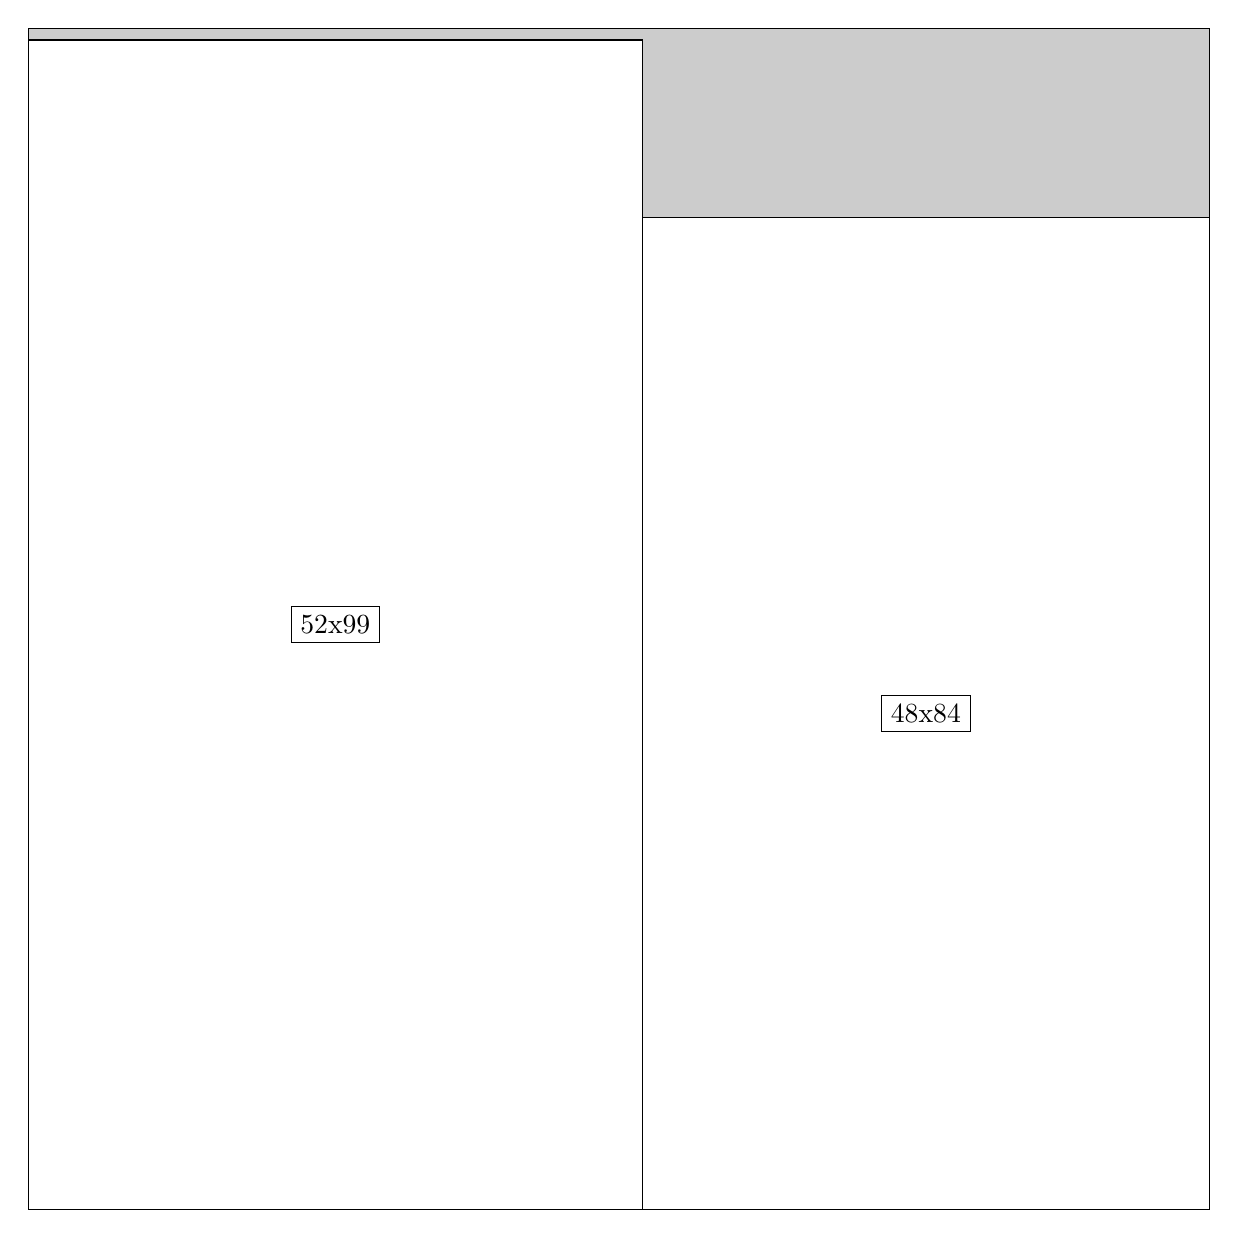
\begin{tikzpicture}[shorten >=1pt,scale=1.0,every node/.style={scale=1.0},->]
\tikzstyle{vertex}=[circle,fill=black!25,minimum size=14pt,inner sep=0pt]
\filldraw[fill=gray!40!white, draw=black] (0,0) rectangle (15.0,15.0);
\foreach \name/\x/\y/\w/\h in {48x84/7.8/0.0/7.199999999999999/12.6,52x99/0.0/0.0/7.8/14.85}
\filldraw[fill=white!40!white, draw=black] (\x,\y) rectangle node[draw] (\name) {\name} ++(\w,\h);
\end{tikzpicture}


w =48 , h =84 , x =52 , y =0 , v =4032
\par
w =52 , h =99 , x =0 , y =0 , v =5148
\par
\newpage


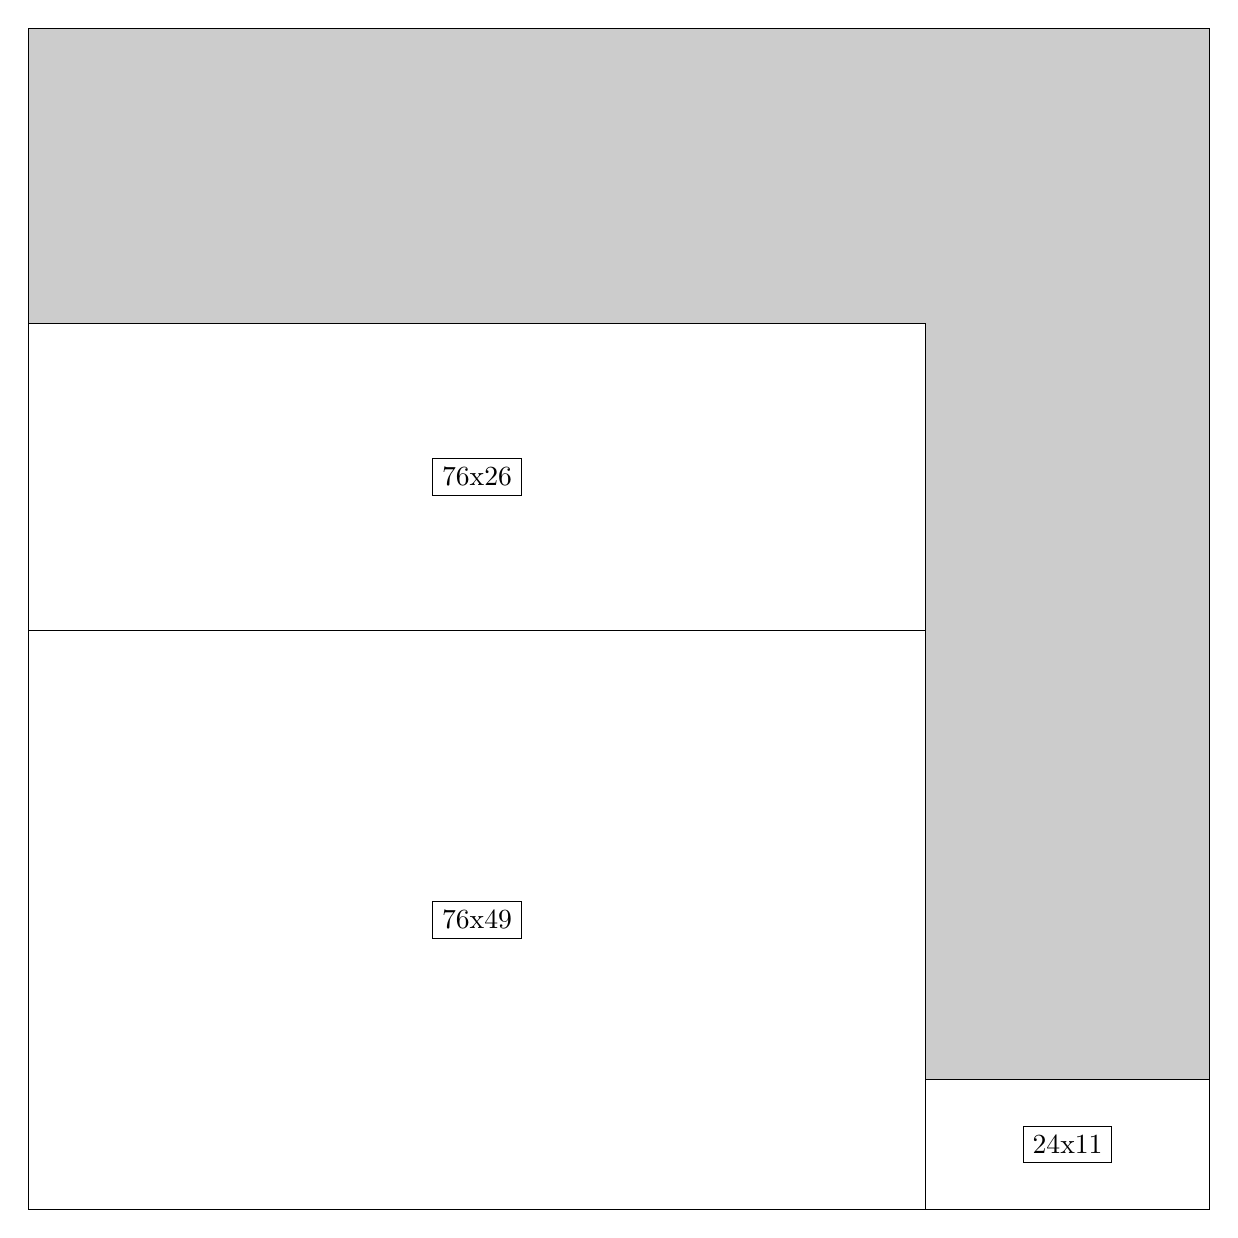
\begin{tikzpicture}[shorten >=1pt,scale=1.0,every node/.style={scale=1.0},->]
\tikzstyle{vertex}=[circle,fill=black!25,minimum size=14pt,inner sep=0pt]
\filldraw[fill=gray!40!white, draw=black] (0,0) rectangle (15.0,15.0);
\foreach \name/\x/\y/\w/\h in {76x49/0.0/0.0/11.4/7.35,76x26/0.0/7.35/11.4/3.9,24x11/11.4/0.0/3.5999999999999996/1.65}
\filldraw[fill=white!40!white, draw=black] (\x,\y) rectangle node[draw] (\name) {\name} ++(\w,\h);
\end{tikzpicture}


w =76 , h =49 , x =0 , y =0 , v =3724
\par
w =76 , h =26 , x =0 , y =49 , v =1976
\par
w =24 , h =11 , x =76 , y =0 , v =264
\par
\newpage


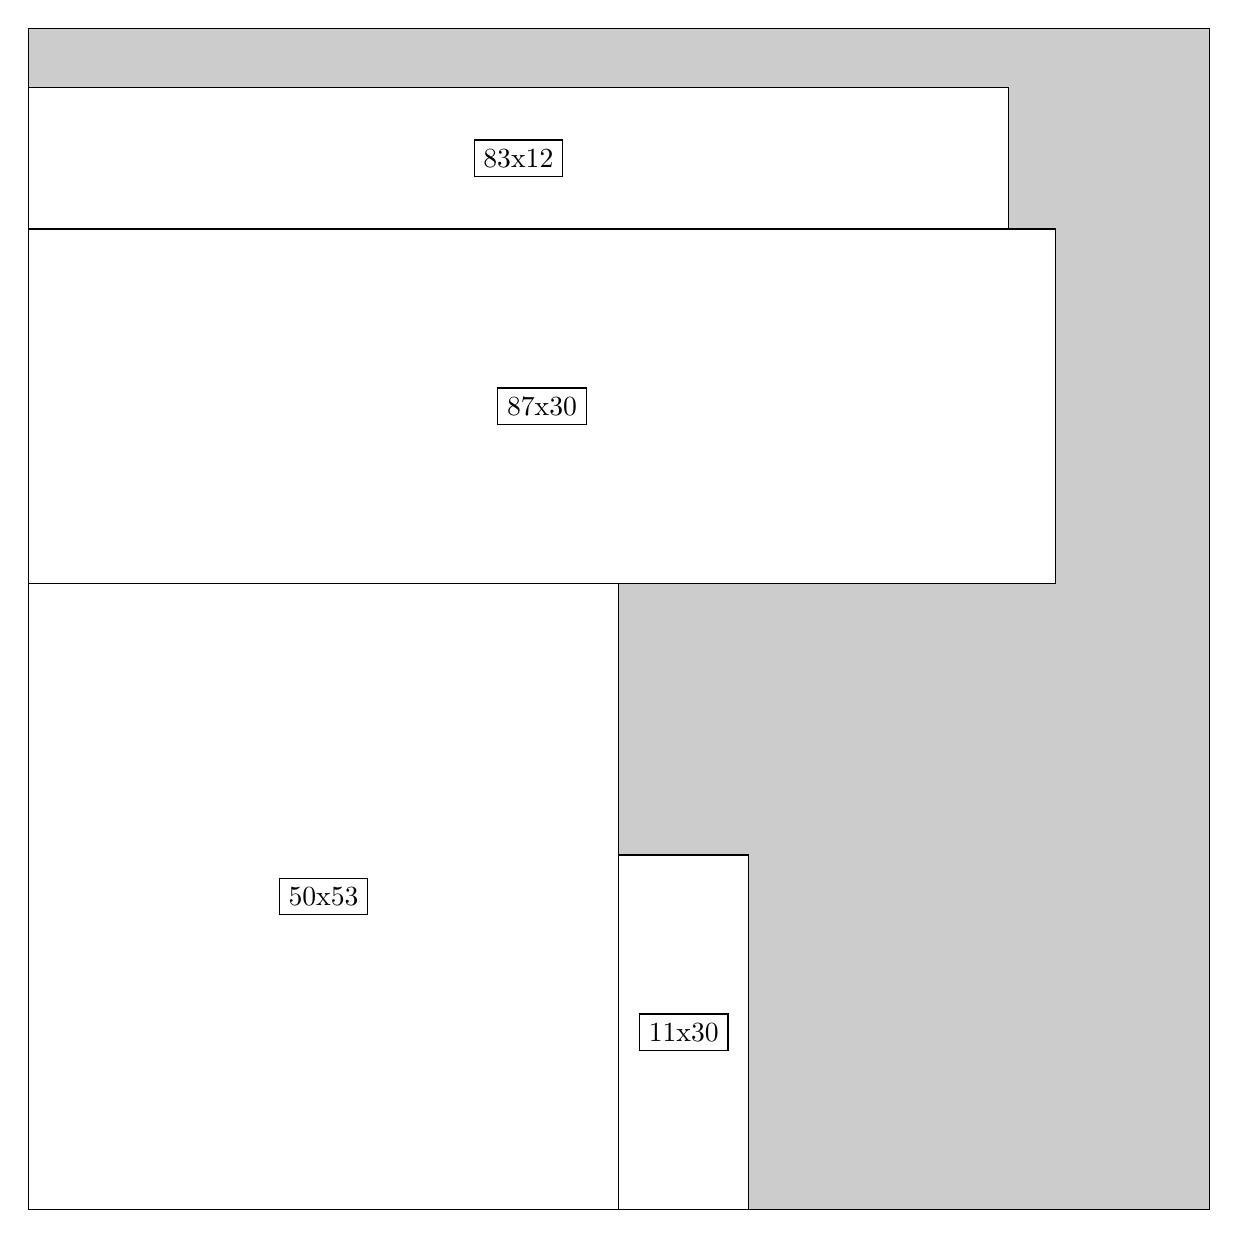
\begin{tikzpicture}[shorten >=1pt,scale=1.0,every node/.style={scale=1.0},->]
\tikzstyle{vertex}=[circle,fill=black!25,minimum size=14pt,inner sep=0pt]
\filldraw[fill=gray!40!white, draw=black] (0,0) rectangle (15.0,15.0);
\foreach \name/\x/\y/\w/\h in {50x53/0.0/0.0/7.5/7.949999999999999,87x30/0.0/7.949999999999999/13.049999999999999/4.5,83x12/0.0/12.45/12.45/1.7999999999999998,11x30/7.5/0.0/1.65/4.5}
\filldraw[fill=white!40!white, draw=black] (\x,\y) rectangle node[draw] (\name) {\name} ++(\w,\h);
\end{tikzpicture}


w =50 , h =53 , x =0 , y =0 , v =2650
\par
w =87 , h =30 , x =0 , y =53 , v =2610
\par
w =83 , h =12 , x =0 , y =83 , v =996
\par
w =11 , h =30 , x =50 , y =0 , v =330
\par
\newpage


\end{document}